%% Short companion; the full deck remains unchanged.
%% Mathematical companion: equations and diagrams, with hidden notes.
%% Compile: tectonic -Z shell-escape talks/zcash-private-transactions-short.tex
\documentclass[aspectratio=169,14pt]{beamer}
\usetheme{default}
\usefonttheme{serif}
\setbeamertemplate{navigation symbols}{}
\setbeamertemplate{itemize items}{\textendash}
\setbeamersize{text margin left=9mm,text margin right=9mm}
\renewcommand{\appendixname}{Appendix}
\usepackage{amsmath,mathtools}
\usepackage{fontspec,unicode-math}
\setmainfont{STIX2Text}[Path=../fonts/, Extension=.otf,
  UprightFont=*-Regular, ItalicFont=*-Italic,
  BoldFont=*-Bold, BoldItalicFont=*-BoldItalic]
\setmathfont{STIX2Math}[Path=../fonts/, Extension=.otf]
\usepackage{array,booktabs}
\usepackage{tikz}
\usetikzlibrary{arrows.meta,positioning,calc,fit,backgrounds}

% A mathematical handout on a slide: one text/math family, ink on white.
\definecolor{arbink}{HTML}{252925}
\definecolor{arb}{HTML}{355E4C}
\definecolor{arbred}{HTML}{943F3B}
\definecolor{arbdim}{HTML}{646C66}
\setbeamercolor{normal text}{fg=arbink,bg=white}
\setbeamercolor{structure}{fg=arb}
\setbeamercolor{frametitle}{fg=arbink}
\setbeamercolor{alerted text}{fg=arbred}
\setbeamercolor{itemize item}{fg=arbdim}
\setbeamercolor{page number in head/foot}{fg=arbdim}
\setbeamerfont{frametitle}{size=\fontsize{18}{22},series=\mdseries}
\setbeamerfont{page number in head/foot}{size=\fontsize{7}{8}}
\setbeamertemplate{frametitle}{%
  \nointerlineskip\vskip3mm
  \begin{beamercolorbox}[wd=\textwidth,sep=0pt]{frametitle}
    \usebeamerfont{frametitle}\strut\insertframetitle\strut\par
    \ifx\insertframesubtitle\empty\else
      {\usebeamerfont{framesubtitle}\usebeamercolor[fg]{framesubtitle}%
        \insertframesubtitle\par}%
    \fi
  \end{beamercolorbox}
  \vskip1mm}
\setbeamertemplate{footline}{%
  \hfill{\usebeamerfont{page number in head/foot}%
    \usebeamercolor[fg]{page number in head/foot}\insertframenumber}%
  \hspace*{9mm}\vskip2mm}
\setbeamertemplate{title page}{%
  \vspace*{14mm}
  {\small\scshape\color{arb}The Zcash Arboretum\par}
  \vskip8mm
  {\fontsize{30}{34}\selectfont\inserttitle\par}
  \vskip4mm
  {\large\color{arbdim}\insertsubtitle\par}
  \vskip10mm
  {\small\insertauthor\par}}
\tikzset{thick/.style={line width=0.6pt},
  very thick/.style={line width=0.85pt}}


% References and supporting explanations are hidden speaker notes.
% To print notes, change "hide notes" to "show notes" and rebuild separately.
\setbeameroption{hide notes}
\setlength{\tabcolsep}{8pt}
\newcommand{\nf}{\ensuremath{\mathsf{nf}}}
\newcommand{\cv}{\ensuremath{\mathsf{cv}}}
\newcommand{\ak}{\ensuremath{\mathsf{ak}}}
\newcommand{\ask}{\ensuremath{\mathsf{ask}}}
\newcommand{\rk}{\ensuremath{\mathsf{rk}}}
\newcommand{\rsk}{\ensuremath{\mathsf{rsk}}}
\title{Zcash for Bitcoiners}
\subtitle{the mathematics of a private transaction}
\author{m@rek.onl}
\date{}
\definecolor{tierfull}{RGB}{210,140,40}
\definecolor{tierin}{RGB}{60,130,180}
\newcommand{\F}{\mathbb F}
\newcommand{\cm}{\mathsf{cm}}
\newcommand{\cmx}{\mathsf{cmx}}
\newcommand{\nk}{\mathsf{nk}}
\newcommand{\ivk}{\mathsf{ivk}}
\newcommand{\gd}{\mathsf{g_d}}
\newcommand{\pkd}{\mathsf{pk_d}}
\newcommand{\rcm}{\mathsf{rcm}}
\newcommand{\Extract}{\mathsf{Extract}}
\newcommand{\NoteCommit}{\mathsf{NoteCommit}}
\newcommand{\PI}{\mathrm{PI}}
\tikzset{
  flow/.style={-{Stealth[length=2mm]},thick,arbdim},
  box/.style={draw=arb!65,inner sep=6pt,align=center},
  labeltext/.style={font=\small,text=arbdim,align=center}
}
\begin{document}

\begin{frame}[plain,t]
\titlepage
\note{A mathematical short route through the Arboretum, not a compressed
catalogue of the full workshop. The slides carry constructions and worked
steps; the speaker supplies the narration. The full deck remains separate.
Source references stay in these hidden notes, never on the slides.}
\end{frame}

\section{Commitments and conservation}
\begin{frame}{Arithmetic with a modulus}
For a prime $p$, the field $\F_p$ is arithmetic modulo $p$.
\[
\F_{97}=\{0,1,\ldots,96\}.
\]
\[
96+2=1,\qquad 5\cdot39=1.
\]
Every nonzero element has an inverse:
\[
5^{-1}=39\quad\text{in }\F_{97}.
\]
\note{Source: Math Guide, Rings and fields; Halo 2 Guide, Worked example.
A field supports addition, subtraction, multiplication and division by
nonzero elements. The small field will return in the proof example.
The actual protocol uses much larger prime fields. Numbers are checked
by check_short_slides.py.}
\end{frame}

\begin{frame}{Curve points and scalars are different objects}
The Pallas curve has equation $y^2=x^3+5$ over $\F_p$.
Its points, including the identity $\mathcal O$, form a group.
\[
[k]P=\underbrace{P+\cdots+P}_{k\text{ additions}},
\qquad [a+b]P=[a]P+[b]P.
\]
\[
\underbrace{p=p_{\mathrm{Pallas}}}_{\text{coordinates}}
\qquad
\underbrace{q=p_{\mathrm{Vesta}}}_{\text{group order; scalars in }\F_q}
\]
\note{Source: Math Guide, Elliptic curves; protocol specification,
Pallas and Vesta. Use integer representatives for scalar multiplication;
the scalar is reduced modulo the prime group order q. Curve addition
is not coordinatewise addition. We abbreviate the two primes only in
this deck. Bitcoiners know the curve-point/public-key distinction.
The identity is the point at infinity.}
\end{frame}

\begin{frame}{Commit to an amount}
Fix public, nonzero curve points $V,R$.
Assume nobody knows $\lambda$ (lambda) with $R=[\lambda]V$.
\[
\boxed{C(v;r)=[v]V+[r]R}
\]
The amount is $v$; the fresh, secret blinder is $r\in\F_q$.
\[
\underbrace{\text{hiding}}_{\text{cannot read }v}
\qquad
\underbrace{\text{binding}}_{\text{cannot change the opening }(v,r)}
\]
\note{Source: Crypto Guide, Pedersen commitments. V and R are the
Orchard value and randomness bases, fixed by hashing to the curve, not
a setup party's retained secret. Binding means no two distinct
openings can feasibly be produced; hiding is information-theoretic
for a uniform blinder. Values are scalars here; integer ranges follow.}
\end{frame}

\begin{frame}{Why it hides}
Multiplication by $R$ permutes all $q$ group points:
\[
r\ \text{uniform in }\F_q
\quad\Longrightarrow\quad
[r]R\ \text{uniform in the group}.
\]
Adding a fixed point only permutes them again:
\[
[v]V+[r]R\ \text{has the same distribution for every }v.
\]
\note{Source: Crypto Guide, Pedersen commitments, perfect hiding.
Because R is nonzero in a prime-order group it generates the group.
This is a bijection argument, not a claim that discrete logarithms
are required for hiding. Fresh independent blinders matter.}
\end{frame}

\begin{frame}{Why it binds}
Suppose two different amounts open the same commitment:
\[
[v_0]V+[r_0]R=[v_1]V+[r_1]R.
\]
Then
\[
[v_0-v_1]V=[r_1-r_0]R
\]
and therefore
\[
\boxed{\lambda=(v_0-v_1)(r_1-r_0)^{-1}\pmod q.}
\]
That would reveal the supposedly unknown relation $R=[\lambda]V$.
\note{Source: Crypto Guide, Pedersen commitments, computational binding.
If v0 differs from v1 in Fq, r1-r0 cannot be zero, so the inverse
exists. This reduction relies on the difficulty of finding the
discrete logarithm between the fixed bases; it does not claim that
such a logarithm fails to exist.}
\end{frame}

\begin{frame}{One Action: one input, one output}
An \emph{Action} pairs an old note with a new note.
A note is a private coin; either side may carry zero value.
\[
\cv_i=[v_{\mathrm{old},i}-v_{\mathrm{new},i}]V+[r_i]R.
\]
\begin{center}
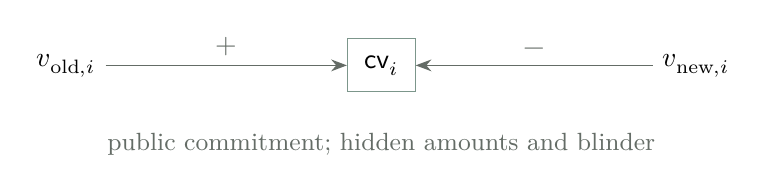
\begin{tikzpicture}[x=1cm,y=1cm]
\node (old) at (0,0) {$v_{\mathrm{old},i}$};
\node[box] (cv) at (4,0) {$\cv_i$};
\node (new) at (8,0) {$v_{\mathrm{new},i}$};
\draw[flow] (old)--node[above] {$+$} (cv);
\draw[flow] (new)--node[above] {$-$} (cv);
\node[labeltext] at (4,-1) {public commitment; hidden amounts and blinder};
\end{tikzpicture}
\end{center}
\note{Source: Ironwood Guide, Value commitments and binding signatures.
Here cv abbreviates cv-net and ri is the Action's value-commitment
randomness rcv. It commits to the signed difference, not to the
entire note. Zero-valued dummy sides permit different real input
and output counts.}
\end{frame}

\begin{frame}{Conservation is a cancellation}
Let $b$ be the public net value leaving the shielded pool.
The public binding key is
\[
\mathsf{bvk}=\sum_i\cv_i-[b]V.
\]
Expanding:
\[
\mathsf{bvk}
=\Bigl[\underbrace{\sum_i(v_{\mathrm{old},i}-v_{\mathrm{new},i})-b}
_{\Delta\text{ (delta): imbalance}}\Bigr]V
+\Bigl[\sum_i r_i\Bigr]R.
\]
\note{Source: Ironwood Guide, Value commitments and binding signatures.
The protocol calls b valueBalance. Its sign is positive for net
value exiting this pool. For a fully shielded single-pool payment,
that exit pays the public fee. The Action proof binds each cv to
the amounts in that Action's actual notes.}
\end{frame}

\begin{frame}{Why the binding signature enforces balance}
A binding signature requires knowing $k$ with $\mathsf{bvk}=[k]R$.
Let $s:=\sum_i r_i$ be the total blinder. Then
\[
[\Delta]V=[k-s]R.
\]
If balanced, $\Delta=0$ and the author knows $k=s$.
\[
\Delta\ne0\quad\Longrightarrow\quad
\lambda=\Delta(k-s)^{-1},
\]
revealing the forbidden relation $R=[\lambda]V$.
\note{Source: Crypto Guide, Value commitments and binding signatures;
Ironwood Guide, Value commitments and binding signatures. This is
RedPallas with R as its base. The algebra alone does not prove
conservation: a signature under the aggregate key supplies knowledge
of its scalar, under the signature security assumptions. For an
unbalanced sum, knowing that scalar and the openings yields the
forbidden relation between V and R.}
\end{frame}

\begin{frame}{Field equality is not yet integer equality}
In a field,
\[
q-1=-1,\qquad q=0.
\]
The proof therefore constrains each note amount to
\[
\boxed{0\le v<2^{64}.}
\]
Bounded values and transaction size prevent a nonzero
integer imbalance from wrapping around modulo $q$.
\note{Source: Ironwood Guide, Value commitments and binding signatures;
Action statement range checks. The circuit also checks the signed
net-value representation. A 64-bit range for each note alone is not
a proof about an unbounded number of notes: the consensus transaction
size bound limits the number of Actions. Public valueBalance has
its own consensus monetary bounds.}
\end{frame}

\section{Notes, membership and authority}
\begin{frame}{A recipient is a curve relation}
A diversifier $d$ selects a public base $\gd$ by hashing to the curve.
The private incoming-viewing scalar is $\ivk$.
\begin{center}
% Lower spine of the Ironwood key-ladder figure.
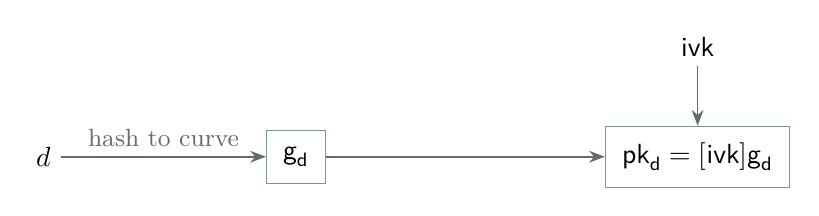
\begin{tikzpicture}[x=1cm,y=1cm]
\node (d) at (0,0) {$d$};
\node[box] (gd) at (3.2,0) {$\gd$};
\node[box] (pkd) at (8.3,0) {$\pkd=[\ivk]\gd$};
\node (ivk) at (8.3,1.4) {$\ivk$};
\draw[flow] (d)--node[above,font=\small] {hash to curve} (gd);
\draw[flow] (gd)--(pkd);
\draw[flow] (ivk)--(pkd);
\end{tikzpicture}
\end{center}
\[
\mathsf{addr}=(d,\pkd).
\]
\note{Source: Ironwood Guide, Diversified addresses and key-ladder figure.
GroupHash uses the fixed Orchard-gd domain. The scalar ivk alone
is not the complete incoming viewing key: that is the pair (dk,ivk),
including the diversifier key. The address-generation branches
dk and ovk are omitted, not incorrectly derived from ivk.}
\end{frame}

\begin{frame}{The private note}
\[
\mathbf n=(\mathsf{addr},v,\rho,\psi,\rcm).
\]
\begin{center}
\renewcommand{\arraystretch}{1.25}
\begin{tabular}{@{}ll@{}}
$\mathsf{addr}=(d,\pkd)$ & recipient \\
$v$ & amount in zatoshi \\
$\rho$ (rho) & uniqueness seed, in $\F_p$ \\
$\psi$ (psi) & additional note randomness, in $\F_p$ \\
$\rcm$ & commitment blinder, in $\F_q$
\end{tabular}
\end{center}
One ZEC is $10^8$ zatoshi.
\note{Source: Ironwood Guide, Notes and note commitments.
The nullifier, defined shortly, is the public spent-note marker.
The wallet reconstructs psi and rcm from the note's random seed
and other note data; they are not independent wire fields. In
Ironwood, rcm also depends on all five commitment-message fields.
This slide gives the abstract note, not its ciphertext encoding.}
\end{frame}

\begin{frame}{From a note to a public leaf}
Write $P^\star$ for an encoded point; $\Vert$ joins bit strings.
The encoding $\mathrm{LE}_k$ has $k$ bits, lowest bit first.
\begin{align*}
m&=\gd^\star\Vert\pkd^\star\Vert\mathrm{LE}_{64}(v)\\
 &\qquad\Vert\mathrm{LE}_{255}(\rho)\Vert\mathrm{LE}_{255}(\psi),\\[2pt]
\cm&=\NoteCommit_{\rcm}(m),\\
\cmx&=\Extract(\cm).
\end{align*}
The note commitment $\cm$ is a point; $\cmx$ is its $x$-coordinate.
Unlike $\cv_i$, $\NoteCommit$ binds the note's full contents.
\note{Source: Ironwood Guide, Notes and note commitments; protocol
specification, Orchard note commitment. NoteCommit is the protocol's
Sinsemilla-based commitment, not the Pedersen value commitment.
Extract maps the identity to zero; otherwise it returns x.
The starred point encoding is 256 bits. The little-endian encodings
in this commitment are 255 bits for rho and psi; they must not be
confused with 256-bit encodings in the randomness derivation.}
\end{frame}

\begin{frame}{Membership without revealing the leaf}
% Native geometry and labels from Ironwood's Merkle-path figure.
\begin{center}
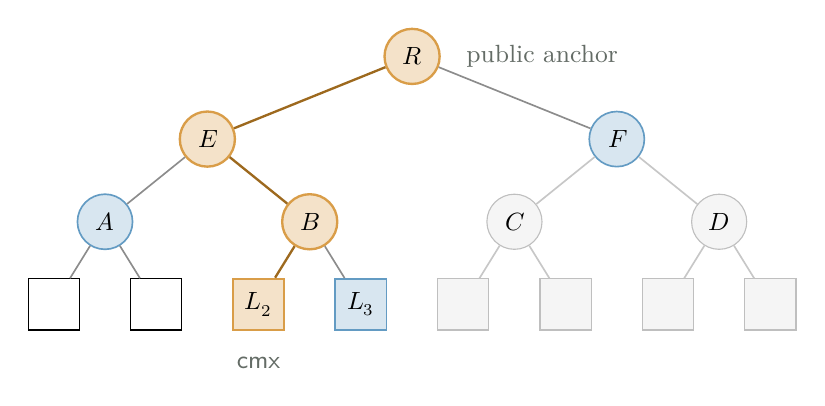
\begin{tikzpicture}[x=1.3cm,y=1.05cm,
  lf/.style={draw,minimum size=6.5mm,inner sep=0pt,font=\small},
  nd/.style={draw,circle,minimum size=7mm,inner sep=0pt,font=\small},
  route/.style={fill=tierfull!25,draw=tierfull!85,very thick},
  sibl/.style={fill=tierin!20,draw=tierin!80,thick},
  faded/.style={draw=black!25,fill=black!4},
  ed/.style={black!45,thick},
  red/.style={draw=tierfull!75!black,very thick},
  fed/.style={black!22,thick}]
\node[lf] (L0) at (0,0) {};
\node[lf] (L1) at (1,0) {};
\node[lf,route] (L2) at (2,0) {$L_2$};
\node[lf,sibl] (L3) at (3,0) {$L_3$};
\node[lf,faded] (L4) at (4,0) {};
\node[lf,faded] (L5) at (5,0) {};
\node[lf,faded] (L6) at (6,0) {};
\node[lf,faded] (L7) at (7,0) {};
\node[nd,sibl] (A) at (.5,1) {$A$};
\node[nd,route] (B) at (2.5,1) {$B$};
\node[nd,faded] (C) at (4.5,1) {$C$};
\node[nd,faded] (D) at (6.5,1) {$D$};
\node[nd,route] (E) at (1.5,2) {$E$};
\node[nd,sibl] (F) at (5.5,2) {$F$};
\node[nd,route] (R) at (3.5,3) {$R$};
\draw[ed] (E)--(A) (B)--(L3) (R)--(F) (A)--(L0) (A)--(L1);
\draw[fed] (F)--(C) (F)--(D) (C)--(L4) (C)--(L5)
  (D)--(L6) (D)--(L7);
\draw[red] (L2)--(B)--(E)--(R);
\node[labeltext,below=2mm of L2] {$\cmx$};
\node[labeltext,right=2mm of R] {public anchor};
\end{tikzpicture}
\end{center}
\centering
Public tree; hidden choice of leaf and path.\\[3pt]
Depth-$3$ illustration; actual depth $32$.
\note{Source: Ironwood Guide, Merkle authentication path figure.
The tree itself is public. The proof hides which leaf and path the
spender uses. The root is called the anchor. Do not suggest the
three-fold toy root is an actual 32-level protocol anchor.}
\end{frame}

\begin{frame}{Three hashes reconstruct the root}
In the illustrated tree, $H_i$ hashes two children at height $i$.
\begin{align*}
B&=H_0(\underbrace{L_2}_{\cmx},L_3),\\
E&=H_1(A,B),\\
R&=H_2(E,F).
\end{align*}
The hidden position is $010_2$; the siblings are $(L_3,A,F)$.
\[
\boxed{R=\mathsf{anchor}.}
\]
\note{Source: Ironwood Guide, Merkle authentication path.
Each position bit chooses left or right at that height. The toy
H0,H1,H2 are not a claim about the protocol's domain-separation tags.
A nonzero spend must reconstruct an allowed public anchor; zero-valued
dummy inputs have a gated membership condition. Anchor admissibility
is an external consensus check, not decided by this equality.}
\end{frame}

\begin{frame}{The spent-note marker is fixed}
The owner's secret nullifier key is $\nk$.
Define $F_{\nk}(\rho)=\mathsf{PoseidonHash}(\nk,\rho)$,
a keyed field hash; $G^{\mathsf{nf}}$ is a fixed public curve point.
\[
\boxed{\nf=\Extract\!\left(
 [F_{\nk}(\rho)+\psi]G^{\mathsf{nf}}+\cm\right).}
\]
The sum is taken in $\F_p$, then read as a scalar; $p<q$.
\medskip

Same note and key $\Longrightarrow$ same \emph{nullifier} $\nf$.
\note{Source: Ironwood Guide, Orchard nullifier; protocol specification,
Nullifier derivation, Orchard. The bracketed sum is reduced in the
Pallas base field, not the scalar field. Its canonical representative
is a scalar because pPallas is less than pVesta. Gnf is the Orchard
K-domain group-hash base. The proof links this nf to the same hidden
note and owner as the membership and authority constraints.}
\end{frame}

\begin{frame}{The proof and the node check different things}
\begin{center}
% Nullifier feedback edge from the Ironwood Action dependency graph.
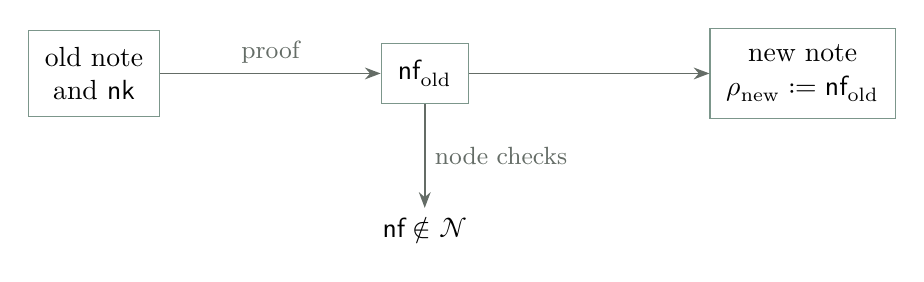
\begin{tikzpicture}[x=1cm,y=1cm]
\node[box] (old) at (0,1) {old note\\and $\nk$};
\node[box] (nf) at (4.2,1) {$\nf_{\mathrm{old}}$};
\node[box] (new) at (9,1) {new note\\$\rho_{\mathrm{new}}:=\nf_{\mathrm{old}}$};
\draw[flow] (old)--node[above,font=\small] {proof} (nf);
\draw[flow] (nf)--(new);
\node (set) at (4.2,-1) {$\nf\notin\mathcal N$};
\draw[flow] (nf)--node[right,font=\small] {node checks} (set);
\end{tikzpicture}
\end{center}
The set $\mathcal N$ contains spent nullifiers.
Reject repeats; insert new ones only when accepting the transaction.
\note{Source: Ironwood Guide, Spending, nullifier uniqueness and Action
dependency figure. Consensus checks both already-spent nullifiers
and duplicates within the proposed transaction or block. Acceptance
is conditional on all validation succeeding, not on this check alone.
The circuit imposes the same-Action rho-new=nf-old linkage.}
\end{frame}

\begin{frame}{The hidden owner links both sides}
Let $\ask$ be the signing secret and $G^{\mathsf{SpendAuth}}$
its fixed public base. The validating key is
\[
\ak=[\ask]G^{\mathsf{SpendAuth}}.
\]
A key commitment with blinder $r_{\ivk}$ links it to the address:
\[
\ivk=\mathsf{CommitIvk}_{r_{\ivk}}\bigl(\Extract(\ak),\nk\bigr),
\qquad
\pkd=[\ivk]\gd.
\]
Same hidden $\ak,\nk$; same note recipient.
\note{Source: Ironwood Guide, Spend-side secrets and Viewing keys;
Action clauses A6 and A7. CommitIvk is the protocol's short
commitment instance, with prescribed input encodings and domain.
The validating key is canonicalised to even y at key generation.
The circuit uses ak, nk, rivk, not ask: a viewing key can prepare a
proof, but signing authority is still supplied separately.}
\end{frame}

\begin{frame}{Randomise the public signing key}
Choose a fresh secret $\alpha$ (alpha), in $\F_q$.
\begin{align*}
\rsk&=\ask+\alpha,\\
\rk&=\ak+[\alpha]G^{\mathsf{SpendAuth}}\\
   &=[\rsk]G^{\mathsf{SpendAuth}}.
\end{align*}
The proof links $\rk$ to the hidden owner.

The spend signature authorises the transaction under $\rk$.
\note{Source: Ironwood Guide, Spend authorisation signatures.
The randomised secret rsk signs the signature digest with RedPallas.
The circuit witnesses alpha and ak, not the signing secret ask.
Proof validity does not replace the spend signature.}
\end{frame}

\begin{frame}{The mathematical statement, not the secret}
\begin{center}
% Focused panel of Ironwood's Action dependency graph.
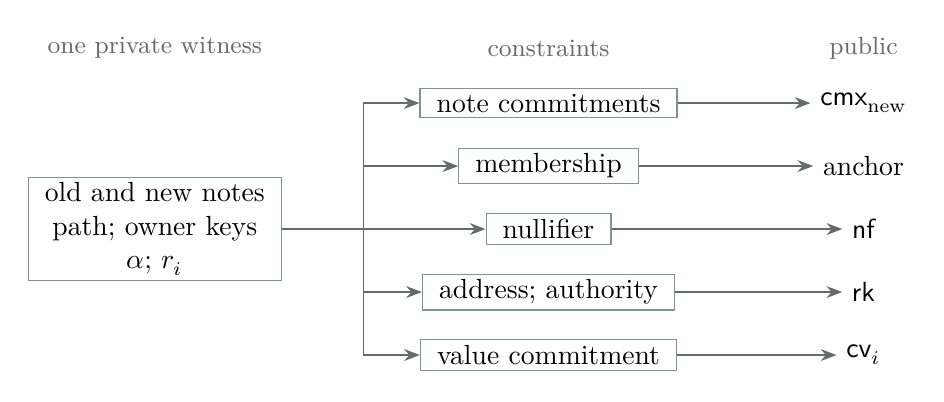
\begin{tikzpicture}[x=1cm,y=1cm,box/.append style={inner ysep=2pt}]
\node[labeltext] at (0,2.3) {one private witness};
\node[labeltext] at (5,2.3) {constraints};
\node[labeltext] at (9,2.3) {public};
\node[box] (w) at (0,0)
  {old and new notes\\path; owner keys\\$\alpha$; $r_i$};
\node[box] (nc) at (5,1.6) {note commitments};
\node[box] (m) at (5,.8) {membership};
\node[box] (nf) at (5,0) {nullifier};
\node[box] (o) at (5,-.8) {address; authority};
\node[box] (c) at (5,-1.6) {value commitment};
\node (cm) at (9,1.6) {$\cmx_{\mathrm{new}}$};
\node (a) at (9,.8) {anchor};
\node (n) at (9,0) {$\nf$};
\node (rk) at (9,-.8) {$\rk$};
\node (cv) at (9,-1.6) {$\cv_i$};
\draw[thick,arbdim] (w.east)--(2.65,0) (2.65,-1.6)--(2.65,1.6);
\foreach \target in {nc,m,nf,o,c}
  \draw[flow] (2.65,0 |- \target.west)--(\target.west);
\draw[flow] (nc)--(cm);
\draw[flow] (m)--(a); \draw[flow] (nf)--(n);
\draw[flow] (o)--(rk); \draw[flow] (c)--(cv);
\end{tikzpicture}
\end{center}
A \emph{witness} is the secret data satisfying the public claim.
Every check uses the same notes and owner keys.
\note{Source: Ironwood Guide, Action statement and dependency figure.
This panel is deliberately a dependency summary for a nonzero spend,
not a complete circuit specification. The same note and owner values
are shared across its constraints. New-note commitment, dummy gates
and cross-address restrictions also belong to the complete Action
statement. Ciphertexts are not constrained by the Action proof.}
\end{frame}

\section{A proof small enough to calculate}
\begin{frame}{A small claim with the same proof machinery}
Use $\F_{97}$ as a toy circuit field. The public claim is:
\[
\text{there exists }x\text{ such that }x^3+x+5=35.
\]
Our private witness is $x=3$.
\[
3\xrightarrow{\text{square}}9
 \xrightarrow{\times3}27
 \xrightarrow{+3}30
 \xrightarrow{+5}35.
\]
\note{Source: Halo 2 Guide, Worked example.
This toy exposes the algebra of a proof; it is not a secure private
claim, since a 97-element witness space is trivially searchable.
The deployed field is much larger. The same arithmetisation approach
handles the actual Action constraints.}
\end{frame}

\begin{frame}{Turn the computation into rows}
The \emph{trace} records intermediate values in columns $a,b,c$.
\begin{center}
\renewcommand{\arraystretch}{1.35}
\begin{tabular}{@{}crrrl@{}}
\toprule
row & $a$ & $b$ & $c$ & constraint\\
\midrule
$0$ & $3$ & $3$ & $9$ & $ab-c=0$\\
$1$ & $9$ & $3$ & $27$ & $ab-c=0$\\
$2$ & $27$ & $3$ & $30$ & $a+b-c=0$\\
$3$ & $30$ & $0$ & $0$ & $a+5-35=0$\\
\bottomrule
\end{tabular}
\end{center}
These private cells are called \emph{advice}.
\note{Source: Halo 2 Guide, Arithmetise the computation.
A constraint is an equation the witness must satisfy. The last row
uses a public input 35; its unused b and c cells happen to be zero in
this witness. This is the exact four-row worked trace.}
\end{frame}

\begin{frame}{One gate, selected differently on each row}
A \emph{gate} is an equation imposed on a row:
\[
q_Mab+q_La+q_Rb+q_Oc+q_C+\PI=0.
\]
The $q$'s are fixed public coefficients, called \emph{selectors}.
The column $\PI$ carries the public input.
\begin{center}
\renewcommand{\arraystretch}{1.2}
\begin{tabular}{@{}crrrrrr@{}}
row & $q_M$ & $q_L$ & $q_R$ & $q_O$ & $q_C$ & $\PI$\\
\midrule
$0,1$ & $1$ & $0$ & $0$ & $-1$ & $0$ & $0$\\
$2$ & $0$ & $1$ & $1$ & $-1$ & $0$ & $0$\\
$3$ & $0$ & $1$ & $0$ & $0$ & $5$ & $-35$
\end{tabular}
\end{center}
\note{Source: Halo 2 Guide, Arithmetise the computation.
Selectors are fixed by the circuit, not chosen to fit the prover's
witness. Public PI is fixed by the statement. Products in the gate
are field operations. The trace and this table are recomputed by
check_short_slides.py.}
\end{frame}

\begin{frame}{Equal values must actually be wired together}
Write $a_i$ for column $a$, row $i$, and likewise for $b,c$.
\begin{center}
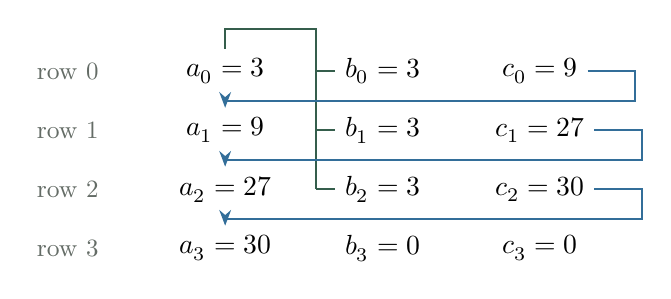
\begin{tikzpicture}[x=1cm,y=1cm]
\foreach \i/\av/\bv/\cvv in {0/3/3/9,1/9/3/27,2/27/3/30,3/30/0/0}{
  \node[labeltext] at (0,-.75*\i) {row $\i$};
  \node (a\i) at (2,-.75*\i) {$a_{\i}=\av$};
  \node (b\i) at (4,-.75*\i) {$b_{\i}=\bv$};
  \node (c\i) at (6,-.75*\i) {$c_{\i}=\cvv$};
}
\draw[very thick,arb] (a0.north) -- ++(0,.25)
  -| (3.15,0) -- (3.15,-1.5);
\foreach \i in {0,1,2}
  \draw[very thick,arb] (3.15,-.75*\i)--(b\i.west);
\draw[flow,tierin!85!black] (c0.east) -- ++(.6,0)
  -- ++(0,-.38) -| (a1.north);
\draw[flow,tierin!85!black] (c1.east) -- ++(.6,0)
  -- ++(0,-.38) -| (a2.north);
\draw[flow,tierin!85!black] (c2.east) -- ++(.6,0)
  -- ++(0,-.38) -| (a3.north);
\end{tikzpicture}
\end{center}
These \emph{copy constraints} are separate from the row gates.
\note{Source: Halo 2 Guide, Arithmetise the computation; Enforcing
the wiring. Green identifies the common x. Blue wires connect each
intermediate result to its next use. Equal numbers in an illustrative
table are not themselves a constraint. Halo 2 separately proves
these equalities with its permutation argument.}
\end{frame}

\begin{frame}{Give the rows multiplicative labels}
Choose $\omega=22$ (omega), with $\omega^2=-1$ and $\omega^4=1$.
\[
H=\{1,22,96,75\}\subset\F_{97}.
\]
\begin{center}
% Adapted roots-of-unity circle: this is a field-operation cycle,
% not a geometric embedding of finite-field residues into C.
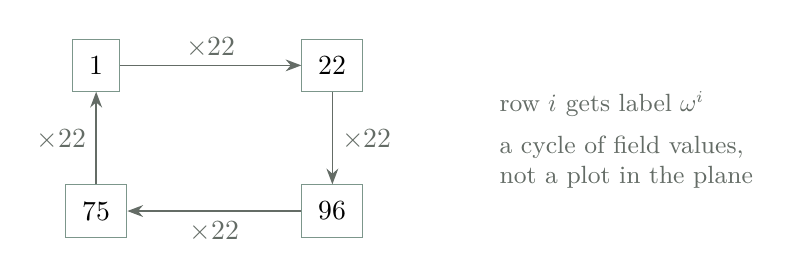
\begin{tikzpicture}[x=1cm,y=1cm]
\node[box] (a) at (0,1.25) {$1$};
\node[box] (b) at (3,1.25) {$22$};
\node[box] (c) at (3,-.6) {$96$};
\node[box] (d) at (0,-.6) {$75$};
\draw[flow] (a)--node[above] {$\times22$} (b);
\draw[flow] (b)--node[right] {$\times22$} (c);
\draw[flow] (c)--node[below] {$\times22$} (d);
\draw[flow] (d)--node[left] {$\times22$} (a);
\node[labeltext,align=left,anchor=west] at (5,.3)
  {row $i$ gets label $\omega^i$\\[4pt]
   a cycle of field values,\\not a plot in the plane};
\end{tikzpicture}
\end{center}
\note{Source: Halo 2 Guide, Interpolate the columns; Math Guide,
Roots of unity, roots-circle figure. Omega is a primitive fourth
root of unity: the four powers are distinct. The diagram adapts the
source's cyclic structure without confusing finite-field residues
with complex points on a unit circle. All arithmetic is modulo 97.}
\end{frame}

\begin{frame}{A column becomes a polynomial}
A \emph{polynomial} is a sum of coefficients times powers of $X$.
Its \emph{degree} is the highest nonzero power.
\[
\boxed{a(X)=90+61X+22X^2+24X^3.}
\]
\begin{center}
\renewcommand{\arraystretch}{1.35}
\begin{tabular}{@{}c|rrrr@{}}
label $h$ & $1$ & $22$ & $96$ & $75$\\
\hline
$a(h)$ & $3$ & $9$ & $27$ & $30$
\end{tabular}
\end{center}
\emph{Interpolation}: four values at distinct labels
determine a unique polynomial of degree $<4$.
\note{Source: Halo 2 Guide, Interpolate the columns; Math Guide,
Lagrange interpolation. Uniqueness follows because the difference
of two degree-less-than-4 polynomials cannot have four distinct
roots unless it is zero. The following root-bound argument relies
on that same fact. This is field interpolation, not a real curve
drawn through four residue values.}
\end{frame}

\begin{frame}{Turn all row gates into one polynomial}
Interpolate every column, including the selectors and $\PI$.
Define the gate residual:
\begin{align*}
G(X)={}&q_M(X)a(X)b(X)\\
      &+q_L(X)a(X)+q_R(X)b(X)\\
      &+q_O(X)c(X)+q_C(X)+\PI(X).
\end{align*}
All row gates hold exactly when
\[
G(h)=0\qquad\text{for every }h\in H.
\]
\note{Source: Halo 2 Guide, All the gates in one polynomial.
G is the residual, the amount by which the equation misses zero.
Its degree is at most 9 because every interpolated column has
degree at most 3. This equivalence concerns the gates only; copy
constraints have a separate polynomial argument.}
\end{frame}

\begin{frame}{Many checks become one divisibility claim}
The \emph{vanishing polynomial} has the row labels as roots (zeros):
\[
Z_H(X):=\prod_{h\in H}(X-h)=X^4-1.
\]
Hence
\[
\boxed{G(h)=0\ \text{for all }h\in H
\iff G(X)=t(X)Z_H(X)}
\]
for a polynomial quotient $t$.
\[
\deg G\le9,\qquad\deg t\le5.
\]
\note{Source: Halo 2 Guide, All the gates in one polynomial;
Math Guide, Polynomial arithmetic. The product sign means multiply
one factor per h in H. A root h gives a factor X-h; the four factors
are distinct. Both implications follow from this factorisation.
The degree bound on t must be enforced, not merely requested.}
\end{frame}

\begin{frame}{Change one cell; the identity breaks}
Replace only $c_0=9$ by $c_0=10$.
The first row now has residual
\[
3\cdot3-10=-1=96\quad\text{in }\F_{97}.
\]
Dividing the altered $G^\ast$ by $Z_H$ leaves
\[
G^\ast=t^\ast Z_H+D,
\qquad
\boxed{D(X)=24(1+X+X^2+X^3)\ne0.}
\]
\note{Source: Halo 2 Guide, What a cheat does to the polynomial and
the random-point worked check. Here t-star is the actual Euclidean
quotient, not an arbitrary malicious quotient. The remainder D has
degree 3. Changing c0 also violates a copy constraint; this example
isolates how the gate check itself catches the error. The complete
numerical derivation is independently recomputed in the slide check.}
\end{frame}

\begin{frame}{A nonzero polynomial has few roots}
For this remainder, the only zeros are $22,75,96$.
\begin{center}
\begin{tikzpicture}[x=.099cm,y=.036cm]
\draw[flow] (0,0)--(102,0) node[right] {$z$};
\draw[flow] (0,0)--(0,104) node[above] {$D(z)$};
\foreach \x in {0,...,96}{
  \pgfmathtruncatemacro{\square}{mod(\x*\x,97)}
  \pgfmathtruncatemacro{\cube}{mod(\square*\x,97)}
  \pgfmathtruncatemacro{\residue}{mod(24*(1+\x+\square+\cube),97)}
  \fill[arb!90] (\x,\residue) circle[radius=1.15pt];
}
\foreach \x in {22,75,96}{
  \draw[tierin!85!black,thick,fill=white] (\x,0) circle[radius=2.2pt];
  \node[below,font=\small,text=tierin!85!black] at (\x,-2) {$\x$};
}
\fill[arbred] (20,53) circle[radius=2.4pt];
\node[above right,font=\small,text=arbred] at (20,53) {$(20,53)$};
\node[left,font=\small] at (0,96) {$96$};
\end{tikzpicture}
\end{center}
For uniform $z\in\F_{97}$, this cheat passes with probability $3/97$.
\note{Source: Halo 2 Guide, The random-point check, numerical remainder
and roots. This discrete residue plot is drawn from the guide's exact
worked polynomial. No lines are drawn between residues. The general
root bound is: a nonzero degree-d polynomial over a field has at most
d roots, by repeated division by X-root. This particular quotient
gives a degree-3 remainder; an arbitrary admissible cheating t gives
degree at most 9 and therefore the weaker general bound 9/97.
This is a toy gate-test probability, not Halo 2's security level.}
\end{frame}

\begin{frame}{One unpredictable point tests the identity}
Fix the polynomials first; then sample $z$.
At $z=20$, the verifier checks
\[
G(z)\stackrel{?}{=}t(z)(z^4-1).
\]
\[
\begin{array}{rcl}
\text{honest:}&75=67\cdot46=75&\pmod{97},\\[4pt]
\text{altered:}&20\ne64&\pmod{97}.
\end{array}
\]
For any nonzero residual of degree at most $9$,
the acceptance probability is at most $9/97$.
\note{Source: Halo 2 Guide, The random-point check.
This probability is for an independent uniform field challenge and
pre-fixed bounded-degree polynomials. The four-row example is
educational, not cryptographically secure. Actual protocol analysis
uses the large field and accounts for all identities, commitment
security, transcript challenges and query bounds.}
\end{frame}

\begin{frame}{Commit to the polynomial before the challenge}
In the real scheme: coefficients in $\F_p$;
points on Vesta, whose group order is $p$.
\[
f(X)=\sum_{i=0}^{d-1}f_iX^i,
\qquad
\boxed{C_f=\sum_{i=0}^{d-1}[f_i]G_i+[r]B.}
\]
The public points $G_i,B$ have no known scalar relation;
the fresh blinder is $r\in\F_p$.
\medskip
An \emph{evaluation proof} establishes $f(z)=y$
for the polynomial fixed by $C_f$.
\note{Source: Halo 2 Guide, Why the prover cannot wriggle;
Crypto Guide, Vector Pedersen commitments.
This is the commitment's algebraic role, not a claim that the tiny
F97 coefficients themselves instantiate the deployed curve scheme.
In the real scheme the polynomial field matches the commitment
group's scalar field; Pallas-coordinate-field polynomials commit on
Vesta. Degree bounds and the blinder are part of the scheme.}
\end{frame}

\begin{frame}{Evaluation is an inner product}
An \emph{inner product} multiplies corresponding entries and adds:
\[
\langle(a_0,\ldots,a_{d-1}),(b_0,\ldots,b_{d-1})\rangle
:=\sum_i a_ib_i.
\]
So
\[
f(z)=\langle(f_0,\ldots,f_{d-1}),(1,z,\ldots,z^{d-1})\rangle.
\]
Halo 2 proves this committed inner-product claim
by repeatedly halving the vectors.
\note{Source: Halo 2 Guide, The inner-product argument.
This identifies the exact claim supplied by the polynomial opening
proof. The logarithmic folding derivation stays in the full deck.
There is no pairing or secret setup exponent. Generator relations
must be unknown, and the blinding coordinate must be accounted for.
The verifier authenticates all evaluations used to reconstruct the
gate identity, not an unbound number called G(z).}
\end{frame}

\begin{frame}{The toy verifier's check}
Prove the evaluations against their commitments:
\[
a(z),\quad b(z),\quad c(z),\quad t(z).
\]
The verifier computes $G(z)$ from these values
and the public selectors and $\PI(z)$, then checks
\[
\boxed{G(z)=t(z)(z^4-1).}
\]
The prover cannot substitute an unrelated $G$.
\note{Source: Halo 2 Guide, The random-point check and Why the prover
cannot wriggle. This is the toy gate identity, before the extra
arguments for copies, lookups and zero knowledge. In this teaching
model selectors are public polynomials, directly evaluable by the
verifier. Real verifier keys also authenticate fixed-polynomial
evaluations through the commitment scheme. All required degree
bounds are part of the committed polynomial relation.}
\end{frame}

\begin{frame}{The order is part of the proof}
\begin{center}
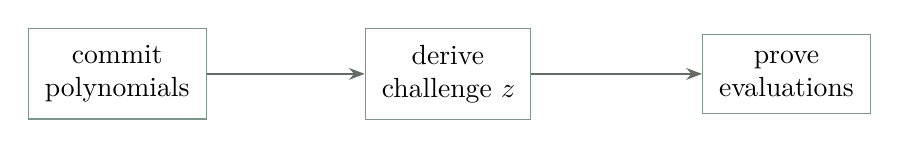
\begin{tikzpicture}[x=1cm,y=1cm]
\node[box] (c) at (0,0) {commit\\polynomials};
\node[box] (z) at (4.2,0) {derive\\challenge $z$};
\node[box] (o) at (8.5,0) {prove\\evaluations};
\draw[flow] (c)--(z);
\draw[flow] (z)--(o);
\end{tikzpicture}
\end{center}
The \emph{transcript} is the public statement and messages so far.
The \emph{Fiat--Shamir transform} derives each challenge by hashing it:
\[
z=\mathsf{HashToField}(\text{transcript}).
\]
Anyone can replay the checks without an interactive verifier.
\note{Source: Halo 2 Guide, Removing the verifier: the Fiat--Shamir
transform. HashToField here denotes the abstract transcript challenge
operation, not the literal deployed function name. Hashing must bind
the full statement and prior messages with proper domain separation.
A prover can try many transcripts; the security argument includes
that query budget. A random-oracle model is an assumption, not an
unconditional identity between hashing and a random coin.}
\end{frame}

\begin{frame}{Binding does not by itself give privacy}
Unblinded evaluations are equations in secret coefficients.
\[
f(z)=f_0+f_1z+\cdots+f_{d-1}z^{d-1}.
\]
Halo 2 adds randomness in two places:
\begin{center}
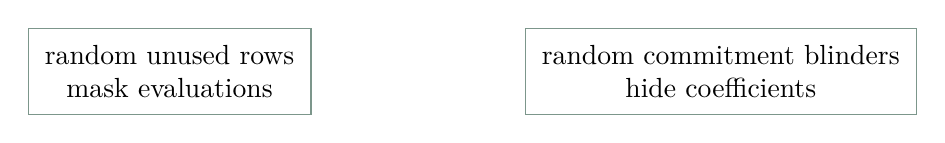
\begin{tikzpicture}[x=1cm,y=1cm]
\node[box] at (0,0) {random unused rows\\mask evaluations};
\node[box] at (7,0) {random commitment blinders\\hide coefficients};
\end{tikzpicture}
\end{center}
\emph{Zero knowledge}: the proof reveals no extra witness information
beyond the public statement.
\note{Source: Halo 2 Guide, Binding the public statement and hiding
the witness. Gates and wiring checks are arranged to ignore the
random rows. Arbitrary extra coefficients would change the active
rows and are not an equivalent construction. Zero knowledge is a
claim about the joint transcript distribution, formalised by a
simulator; fresh randomness in just one isolated component is not
by itself a complete proof of it.}
\end{frame}

\begin{frame}{Back to the transaction}
\begin{center}
\renewcommand{\arraystretch}{1.55}
\begin{tabular}{@{}ll@{}}
\textcolor{arb}{Proof} & hidden notes satisfy the equations\\
\textcolor{arb}{Spend signatures} & owners authorise this transaction\\
\textcolor{arb}{Binding signature} & committed amounts balance\\
\textcolor{arb}{Node state} & anchor allowed; nullifiers unused
\end{tabular}
\end{center}
\medskip
No single equation replaces the other checks.
\note{Source: Ironwood Guide, Verification and Action statement;
Halo 2 Guide, worked example. This returns from the illustrative
gate polynomial to the real proof's job. Actual validation also
includes encodings, amounts, flags, proof parsing, transaction
structure and all other consensus rules. The scope here is the
mathematical core, not a substitute consensus checklist.}
\end{frame}

\end{document}
